% !TEX TS-program = pdflatex
% !TEX encoding = UTF-8 Unicode

% This is a simple template for a LaTeX document using the "article" class.
% See "book", "report", "letter" for other types of document.

\documentclass[12pt]{article} % use larger type; default would be 10pt

\usepackage[utf8]{inputenc} % set input encoding (not needed with XeLaTeX)

%%% Examples of Article customizations
% These packages are optional, depending whether you want the features they provide.
% See the LaTeX Companion or other references for full information.

%%% PAGE DIMENSIONS
\usepackage{geometry} % to change the page dimensions
\geometry{a4paper} % or letterpaper (US) or a5paper or....
% \geometry{margin=2in} % for example, change the margins to 2 inches all round
% \geometry{landscape} % set up the page for landscape
%   read geometry.pdf for detailed page layout information
\setlength{\parindent}{0pt}


% \usepackage[parfill]{parskip} % Activate to begin paragraphs with an empty line rather than an indent

%%% PACKAGES
\usepackage{booktabs} % for much better looking tables
\usepackage{array} % for better arrays (eg matrices) in maths
\usepackage{paralist} % very flexible & customisable lists (eg. enumerate/itemize, etc.)
\usepackage{verbatim} % adds environment for commenting out blocks of text & for better verbatim
\usepackage{subfig} % make it possible to include more than one captioned figure/table in a single float
\usepackage{amsmath} %amsmath is part of AMS-LATEX bundles
\usepackage{amssymb}%symble
\usepackage{amsfonts}%font
\usepackage{amsthm}%provide theorem package
\usepackage{graphicx}
\usepackage{listings}
% These packages are all incorporated in the memoir class to one degree or another...
\usepackage[retainorgcmds]{IEEEtrantools} %In order to use IEEEeqnarray Environment
\usepackage{graphicx} % support the \includegraphics command and options
%\usepackage{indentfirst}%

%%% HEADERS & FOOTERS
\usepackage{fancyhdr} % This should be set AFTER setting up the page geometry
\pagestyle{fancy} % options: empty , plain , fancy
\renewcommand{\headrulewidth}{0pt} % customise the layout...
\lhead{}\chead{}\rhead{}
\lfoot{}\cfoot{\thepage}\rfoot{}

%%% SECTION TITLE APPEARANCE
\usepackage{sectsty}
\allsectionsfont{\sffamily\mdseries\upshape} % (See the fntguide.pdf for font help)
% (This matches ConTeXt defaults)

%%% ToC (table of contents) APPEARANCE
\usepackage[nottoc,notlof,notlot]{tocbibind} % Put the bibliography in the ToC
\usepackage[titles,subfigure]{tocloft} % Alter the style of the Table of Contents
\renewcommand{\cftsecfont}{\rmfamily\mdseries\upshape}
\renewcommand{\cftsecpagefont}{\rmfamily\mdseries\upshape} % No bold!

%%%DEFINE UPRIGHT FONT MISSING FUNCTIONS????????????????????
\DeclareMathOperator{\argh}{argh}
\DeclareMathOperator*{\nut}{Nut}

%%%DEFINE NEW COMMANDS
\newcommand{\ud}{\,\mathrm{d}}

%%%DEFINE THEOREM
%\theoremstyle{definition} 
\theoremstyle{definition}\newtheorem{law}{Law}
\theoremstyle{plain}\newtheorem{jury}[law]{Jury}
\theoremstyle{remark}\newtheorem{juu}{Juu}
\theoremstyle{definition}\newtheorem{kuu}[law]{Kuu}
\theoremstyle{definition}\newtheorem{muu}{Muu}[section]
\theoremstyle{definition}\newtheorem{honoluu}{Honoluu}[section]
\theoremstyle{definition}\newtheorem{konoluu}[muu]{Konoluu}

%%% END Article customizations

%%% The "real" document content comes below...

\title{\textbf{ \begin{LARGE}Artificial Intelligence\end{LARGE}}\\ [0ex]\begin{Large} Homework 3 \end{Large} }
\author{Ning Ma}
\date{} % Activate to display a given date or no date (if empty),
         % otherwise the current date is printed 

\begin{document}
\maketitle
{\bf 3.1}
\begin{equation}
P(Y_1, Y_2, Y_3|X)=P(Y_1|X)P(Y_2|X)P(Y_3|X)
\end{equation}
\begin{equation}
P(Z_1|Y_1, Y_2, Y_3)=P(Z_1|Y_1, Y_2)
\end{equation}
\begin{equation}
P(Z_2|Y_1, Y_2, Y_3)=P(Z_2|Y_2, Y_3)\\
\end{equation}

Thus, the CPTs for the polytree is the following:
\begin{table}[htb]
\caption{CPTs for the polytree}
\centering
\begin{tabular}{|c|c|c|c|c|c|c|c|}
\hline
$Y_1$ & $Y_2$ & $Y_3$ & $Y$ & $P(Y|X=0)$ & $P(Y|X=1)$ & $P(Z_1=1|Y)$ & $P(Z_2=1|Y)$\\
\hline
0 & 0 & 0 & 1 & 0.021 & 0.08 & 0.8 & 0.1\\
\hline
1 & 0 & 0 & 2 & 0.049 & 0.08 & 0.7 & 0.1\\
\hline
0 & 1 & 0 & 3 & 0.009 & 0.32 & 0.6 & 0.2\\
\hline
0 & 0 & 1 & 4 & 0.189 & 0.02 & 0.8 & 0.3\\
\hline
1 & 1 & 0 & 5 & 0.021 & 0.32 & 0.5 & 0.2\\
\hline
1 & 0 & 1 & 6 & 0.441 & 0.02 & 0.7 & 0.3\\
\hline
0 & 1 & 1 & 7 & 0.081 & 0.08 & 0.6 & 0.4\\
\hline
1 & 1 & 1 & 8 & 0.189 & 0.08 & 0.5 & 0.4\\
\hline
\end{tabular}
\label{table:CPTsPolytree}
\end{table}\\

\textbf{3.2}
\begin{enumerate}
\item[(a)]
\begin{equation}
P(X)=\frac{C(x)}{T}
\end{equation}
\begin{equation}
P(Y|X)=\frac{C(x,y)}{C(x)}
\end{equation}
\begin{equation}
P(Z|Y)=\frac{C(x,y)}{C(y)}
\end{equation}

\item[(b)]
\begin{equation}
P(Z)=\frac{C(z)}{T}
\end{equation}

\begin{equation}
P(Y|Z)=\frac{C(y,z)}{C(z)}
\end{equation}

\begin{equation}
P(X|Y)=\frac{C(x,y)}{C(y)}
\end{equation}

\item[(c)] 
For left DAG, we have 
\begin{equation}
P_l(X, Y, Z)=P(X)P(Y|X)P(Z|Y)=\frac{C(x, y)C(y, z)}{TC(y)}
\end{equation}
For the right DAG, we have
\begin{equation}
P_r(X, Y, Z)=P(Z)P(Y|Z)P(X|Y)=\frac{C(y, z)C(x, y)}{TC(y)}=P_l(X, Y, Z)	
\end{equation}
Thus, different DAGs give the same joint distribution
\item[(d)]
No. The only conditional independent relation is $P(X|Y, Z)=P(X|Y)$. This relation is implied by both DAGs.
\end{enumerate}

\textbf{3.3}
\begin{enumerate}
\item[(a)]
See the table printed out.
\lstinputlisting{outputtable_a}

\item[(b)]
See the table printed out.
\lstinputlisting{outputtable_b}

\item[(c)]
I got the following message from Matlab:\\
Logrithm of unigram is $L_u= -57.19869441$\\
Logrithm of bigram is $L_b= -38.09758270$\\
Thus, the bigram model yields the highest log-likelihood.

\item[(d)] I got the following results from Matlab:\\
Logrithm of unigram is $L_u = -44.23642999$\\
Pairs of adjacent words OFFICIALS follows FOURTEEN are not observed. Pairs of adjacent words FIRE follows SOLD are not observed. \\
Since the condictional probability corresponding to these two adjacent words are zero, $L_b$ goes to negative infinite.

\item[(e)] I got the following results from Matlab:\\
maximum value is -42.95806624 with lemda 0.34100000. Thus, the maximum log-likelihood is -42.95806624 with the $\lambda$=0.34. The plot of the log-likelihood as function of $\lambda$ is
\begin{figure}[htbp]
\centering
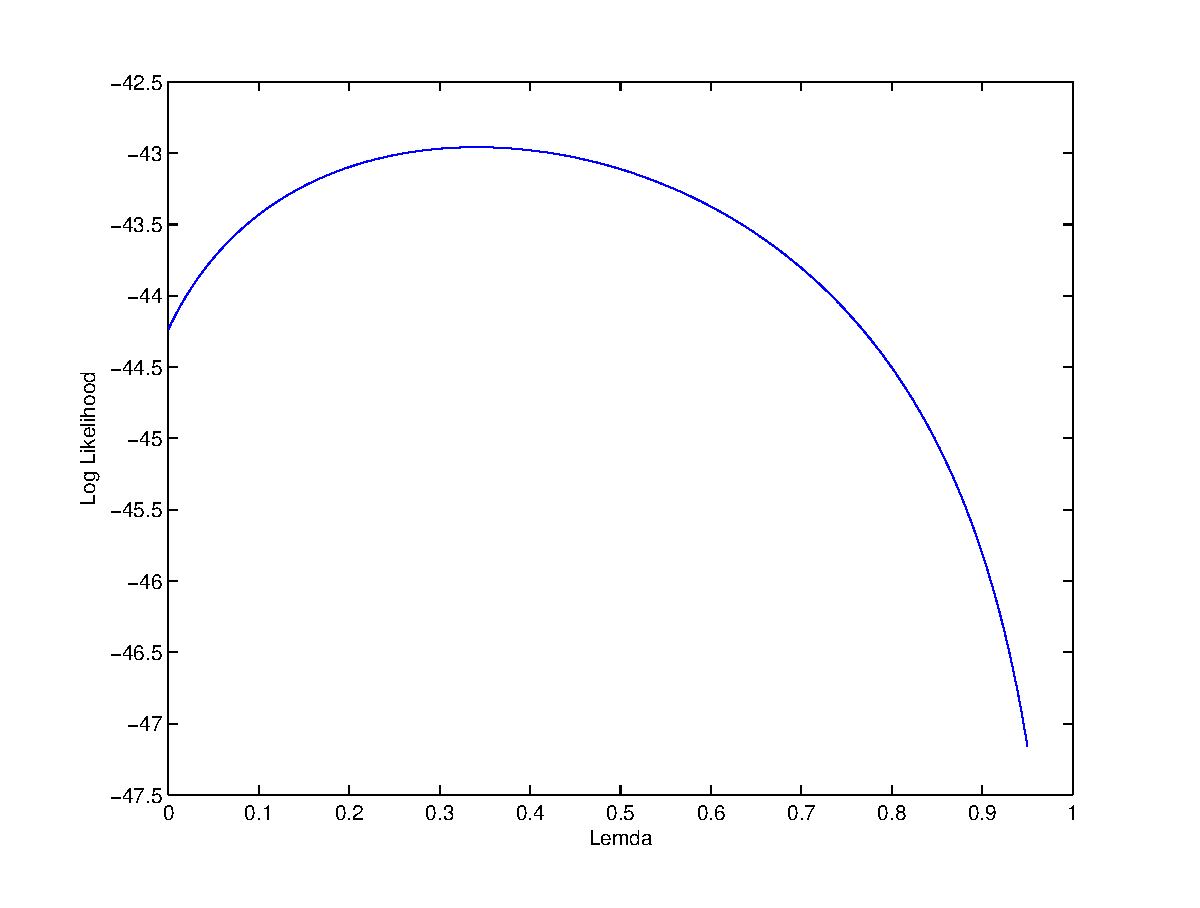
\includegraphics[width=0.8\textwidth]{cse_hw3_e.eps}
\caption{Log-likelihood as fuction of $\lambda$}
\label{LLH1}
\end{figure}
\end{enumerate}
The following is the Matlab source code\\
\\
\lstinputlisting{cse_hm_3total.m}

%P(X_1<X_2<X_3)=\int
%\\
%\textbf{5.3.2} Let $X$ and $Y$ be independent random variables, with $E(X)=1, E(Y)=2, Var(Y)=4.$\\
%\indent \setlength{\hangindent}{2em} (a) FInd $E(10X^2+8Y^2-XY+8X+5Y-1)$\\
%\indent \setlength{\hangindent}{2em} (b) Assuming all variables are normally distributed, find$ P(2X>3Y-5)$
%More text. 
\end{document}
